\documentclass{article}
\usepackage[backend=biber,natbib=true,style=alphabetic,maxbibnames=50]{biblatex}
\addbibresource{/home/nqbh/reference/bib.bib}
\usepackage[utf8]{vietnam}
\usepackage{tocloft}
\renewcommand{\cftsecleader}{\cftdotfill{\cftdotsep}}
\usepackage[colorlinks=true,linkcolor=blue,urlcolor=red,citecolor=magenta]{hyperref}
\usepackage{amsmath,amssymb,amsthm,float,graphicx,mathtools,tikz}
\usetikzlibrary{angles,calc,intersections,matrix,patterns,quotes,shadings}
\allowdisplaybreaks
\newtheorem{assumption}{Assumption}
\newtheorem{baitoan}{}
\newtheorem{cauhoi}{Câu hỏi}
\newtheorem{conjecture}{Conjecture}
\newtheorem{corollary}{Corollary}
\newtheorem{dangtoan}{Dạng toán}
\newtheorem{definition}{Definition}
\newtheorem{dinhly}{Định lý}
\newtheorem{dinhnghia}{Định nghĩa}
\newtheorem{example}{Example}
\newtheorem{ghichu}{Ghi chú}
\newtheorem{hequa}{Hệ quả}
\newtheorem{hypothesis}{Hypothesis}
\newtheorem{lemma}{Lemma}
\newtheorem{luuy}{Lưu ý}
\newtheorem{nhanxet}{Nhận xét}
\newtheorem{notation}{Notation}
\newtheorem{note}{Note}
\newtheorem{principle}{Principle}
\newtheorem{problem}{Problem}
\newtheorem{proposition}{Proposition}
\newtheorem{question}{Question}
\newtheorem{remark}{Remark}
\newtheorem{theorem}{Theorem}
\newtheorem{vidu}{Ví dụ}
\usepackage[left=1cm,right=1cm,top=5mm,bottom=5mm,footskip=4mm]{geometry}
\def\labelitemii{$\circ$}
\DeclareRobustCommand{\divby}{%
	\mathrel{\vbox{\baselineskip.65ex\lineskiplimit0pt\hbox{.}\hbox{.}\hbox{.}}}%
}

\title{Problem: 1st-Order Function -- Bài Tập: Hàm Số Bậc Nhất $y = ax + b$, $a\ne0$}
\author{Nguyễn Quản Bá Hồng\footnote{Independent Researcher, Ben Tre City, Vietnam\\e-mail: \texttt{nguyenquanbahong@gmail.com}; website: \url{https://nqbh.github.io}.}}
\date{\today}

\begin{document}
\maketitle
\tableofcontents

%------------------------------------------------------------------------------%

\section{Mở Đầu Về Phương Trình. Phương Trình Bậc Nhất 1 Ẩn. Phương Trình Thu Gọn Được Về Dạng $ax + b = 0$}

\begin{baitoan}[\cite{Tuyen_Toan_8}, VD27, p. 41]
	Cho phương trình $\dfrac{3(2x + 1)}{4} - \dfrac{5x + 3}{6} = \dfrac{2x - 1}{3} + \dfrac{m}{12}$, $m$: tham số. Tìm giá trị của $m$ để phương trình này có nghiệm.
\end{baitoan}

\begin{baitoan}[\cite{Tuyen_Toan_8}, VD28, p. 41]
	Giải \& biện luận phương trình theo tham số $m$: $\dfrac{m^2}{8}\left[(x + 2)^2 - (x  - 2)^2\right] - 4x = (m - 1)^2 + 3(2m + 1)$.
\end{baitoan}

\begin{baitoan}[\cite{Tuyen_Toan_8}, 181., p. 42]
	Cho 3 phương trình: $(x + 5)(2x - 1) = 0$, $(x + 5)(2x - 1)(x^2 - 3) = 0$, $(x + 5)(x^2 - 3) = 0$. Xét xem trong 3 phương trình này, có 2 phương trình nào tương đương không nếu: (a) $x$ nhận giá trị trên tập $\mathbb{R}$. (b) $x$ nhận giá trị trên tập $\mathbb{Q}$. (c) $x$ nhận giá trị trên tập $\mathbb{Z}$. (d) $x$ nhận giá trị trên tập $\mathbb{N}$.
\end{baitoan}

\begin{baitoan}[\cite{Tuyen_Toan_8}, 182., p. 42]
	Tìm giá trị của hằng số $a$ để phương trình sau vô nghiệm: $\dfrac{a(3x - 1)}{5} - \dfrac{6x - 17}{4} + \dfrac{3x + 2}{10} = 0$.
\end{baitoan}

\begin{baitoan}[\cite{Tuyen_Toan_8}, 183., p. 42]
	Giải phương trình: (a) $\dfrac{x + 3}{1} + \dfrac{2x + 3}{3} + \dfrac{3x + 5}{5} + \cdots + \dfrac{20x + 39}{39} = 22 + \dfrac{4}{3} + \dfrac{6}{5} + \cdots + \dfrac{40}{39}$. (b) $(x - 20) + (x - 19) + (x - 18) + \cdots + 100 + 101 = 101$.
\end{baitoan}

\begin{baitoan}[\cite{Tuyen_Toan_8}, 184., p. 42]
	Giải phương trình: (a) $\left(\dfrac{1}{1\cdot2} + \dfrac{1}{2\cdot3} + \dfrac{1}{3\cdot4} + \cdots + \dfrac{1}{9\cdot10}\right)(x - 1) + \dfrac{x}{10} = x - \dfrac{9}{10}$.\\(b) $\left(\dfrac{1}{1\cdot51} + \dfrac{1}{2\cdot52} + \dfrac{1}{3\cdot53} + \cdots + \dfrac{1}{10\cdot60}\right)x = \dfrac{1}{1\cdot11} + \dfrac{1}{2\cdot12} + \dfrac{1}{3\cdot13} + \cdots +\dfrac{1}{50\cdot60}$.
\end{baitoan}

\begin{baitoan}[\cite{Tuyen_Toan_8}, 185., p. 42]
	Giải \& biện luận phương trình theo tham số $m$: (a) $\dfrac{mx + 5}{10} + \dfrac{x + m}{4} = \dfrac{m}{20}$. (b) $\dfrac{x - 4m}{m + 1} + \dfrac{x - 4}{m - 1} = \dfrac{x - 4m - 3}{m^2 - 1}$.
\end{baitoan}

\begin{baitoan}[\cite{Tuyen_Toan_8}, 186., p. 42]
	Giải \& biện luận phương trình chứa 3 tham số $a,b,c$: (a) $\dfrac{x - a}{bc} + \dfrac{x - b}{ca} + \dfrac{x - c}{ab} = 2\left(\dfrac{1}{a} + \dfrac{1}{b} + \dfrac{1}{c}\right)$. (b) $\dfrac{x - ab}{a + b} + \dfrac{x - bc}{b + c} + \dfrac{x - ca}{c + a} = a + b + c$.
\end{baitoan}

%------------------------------------------------------------------------------%

\section{Phương Trình Tích}
Giải phương trình:

\begin{baitoan}[\cite{Tuyen_Toan_8}, VD29, p. 43]
	$\dfrac{x + 16}{49} + \dfrac{x + 18}{47} = \dfrac{x + 20}{45} - 1$.
\end{baitoan}

\begin{baitoan}[\cite{Tuyen_Toan_8}, 187., p. 43]
	 (a) $x^3 - 3x^2 + 4 = 0$. (b) $x^4 + x^3 - 4x^2 + 5x - 3 = 0$.
\end{baitoan}

\begin{baitoan}[\cite{Tuyen_Toan_8}, 188., p. 43]
	(a) $(2x^2 - 3x - 1)^2 - 3(2x^2 - 3x - 5) - 16 = 0$. (b) $x(x - 1)(x + 4)(x + 5) = 84$.
\end{baitoan}

\begin{baitoan}[\cite{Tuyen_Toan_8}, 189., p. 44]
	(a) $\dfrac{x + 43}{57} + \dfrac{x + 46}{54} = \dfrac{x + 49}{51} + \dfrac{x + 52}{48}$. (b) $\dfrac{x - 69}{30} + \dfrac{x - 67}{32} + \dfrac{x - 65}{34} = \dfrac{x - 63}{36} + \dfrac{x - 61}{38} + \dfrac{x - 59}{40}$.
\end{baitoan}

\begin{baitoan}[\cite{Tuyen_Toan_8}, 190., p. 44]
	(a) $\dfrac{x - 17}{33} + \dfrac{x - 21}{29} + \dfrac{x}{25} = 4$. (b) $\dfrac{148 - x}{25} + \dfrac{169 - x}{23} + \dfrac{180 - x}{21} + \dfrac{199 - x}{19} = 10$.
\end{baitoan}

\begin{baitoan}[\cite{Tuyen_Toan_8}, 191., p. 44]
	(a) $(2x - 5)^3 - (3x - 4)^3 + (x + 1)^3 = 0$. (b) $(x - 1)^3 + (2x - 3)^3 + (3x - 5)^3 - 3(x - 1)(2x - 3)(3x - 5) = 0$. (c) $(x^2 + 3x - 4)^3 + (3x^2 + 7x + 4)^3 = (4x^2 + 10x)^3$.
\end{baitoan}

\begin{baitoan}[\cite{Tuyen_Toan_8}, 192., p. 44]
	(a) $(x + 5)^4 + (x - 4)^4 = (2x + 1)^4$. (b) $(x - 4)^4 + (x - 2)^4 = 82$.
\end{baitoan}

\begin{baitoan}[\cite{Tuyen_Toan_8}, 193., p. 44]
	(a) $x(x + 2) + a^2 - 3 = 2a(x + 1)$. (b) $x^3 - (a + b + c)x^2 + (ab + bc + ca)x - abc = 0$. (c) $x^3 + 3ax^2 + 3(a^2 - bc)x + a^3 + b^3 + c^3 - 3abc = 0$.
\end{baitoan}

%------------------------------------------------------------------------------%

\section{Phương Trình Chứa Ẩn Ở Mẫu Thức}

\begin{baitoan}[\cite{Tuyen_Toan_8}, VD30, p. 45]
	Giải phương trình: $\left(\dfrac{x + 3}{x - 2}\right)^2 + 6\left(\dfrac{x - 3}{x + 2}\right)^2 - \dfrac{7(x^2 - 9)}{x^2 - 4} = 0$.
\end{baitoan}

\begin{baitoan}[\cite{Tuyen_Toan_8}, VD31, p. 45]
	Giải \& biện phương trình theo tham số $m$: $\dfrac{x - m}{x + 5} + \dfrac{x - 5}{x + m} = 2$.
\end{baitoan}
Giải phương trình:

\begin{baitoan}[\cite{Tuyen_Toan_8}, 194., p. 46]
	(a) $\dfrac{x + 1}{x + 2} + \dfrac{5}{x - 2} = \dfrac{4}{x^2 - 4} + 1$. (b) $\dfrac{x - 1}{x^2 - x + 1} - \dfrac{x + 1}{x^2 + x + 1} = \dfrac{10}{x(x^4 + x^2 + 1)}$.
\end{baitoan}

\begin{baitoan}[\cite{Tuyen_Toan_8}, 195., p. 46]
	(a) $\dfrac{x + 9}{10} + \dfrac{x + 10}{9} = \dfrac{9}{x + 10} + \dfrac{10}{x + 9}$. (b) $\dfrac{x^2 - 2x + 2}{x - 1} + \dfrac{x^2 - 8x + 20}{x - 4} = \dfrac{x^2 - 4x + 6}{x - 2} + \dfrac{x^2 - 6x + 12}{x - 3}$.
\end{baitoan}

\begin{baitoan}[\cite{Tuyen_Toan_8}, 196., p. 46]
	(a) $\dfrac{x - 5}{x - 5} + \dfrac{x - 6}{x - 5} + \dfrac{x - 7}{x - 5} + \cdots + \dfrac{1}{x - 5} = 4$. (b) $\dfrac{1}{x^2 + 3x + 2} + \dfrac{1}{x^2 + 5x + 6} + \dfrac{1}{x^2 + 7x + 12} + \cdots + \dfrac{1}{x^2 + 15x + 56} = \dfrac{1}{14}$. (c) $\left(1 + \dfrac{1}{1\cdot3}\right)\left(1 + \dfrac{1}{2\cdot4}\right)\left(1 + \dfrac{1}{3\cdot5}\right)\cdots\left(1 + \dfrac{1}{x(x + 2)}\right) = \dfrac{31}{16}$.
\end{baitoan}
Giải \& biện luận phương trình:

\begin{baitoan}[\cite{Tuyen_Toan_8}, 197., p. 47]
	$\dfrac{a}{1 + bx} = \dfrac{b}{1 + ax}$ với tham số $a,b\in\mathbb{R}$, $ab\ne0$.
\end{baitoan}

\begin{baitoan}[\cite{Tuyen_Toan_8}, 198., p. 47]
	$\dfrac{1}{x} - \dfrac{1}{a} + \dfrac{1}{b} = \dfrac{1}{x - a + b}$ với tham số $a,b\in\mathbb{R}$.
\end{baitoan}

\begin{baitoan}[\cite{Tuyen_Toan_8}, 199., p. 47]
	$\dfrac{3}{x - m} - \dfrac{1}{x - 2} = \dfrac{2}{x - 2m}$ với tham số $m\in\mathbb{R}$.
\end{baitoan}

%------------------------------------------------------------------------------%

\section{Giải Bài Toán Bằng Cách Lập Phương Trình}

\begin{baitoan}[\cite{Tuyen_Toan_8}, VD32, p. 47]
	1 sà lan xuôi dòng từ A đến B mất $2.5$ giờ \& ngược dòng từ B về A mất $4$ giờ. Biết vận tốc dòng nước là {\rm3 km{\tt/}h}, tính khoảng cách AB.
\end{baitoan}

\begin{baitoan}[\cite{Tuyen_Toan_8}, 200., p. 48]
	Lúc {\rm7:00}, 1 người đi xe máy từ A đến B dài {\rm45 km}. Tới B, người đó giải quyết xong công việc trong $1$ giờ $30$ phút rồi quay ngay về, tới A lúc {\rm11:00}. Đoạn đường AB gồm 1 đoạn đường bằng \& 1 đoạn lên dốc. Vận tốc lúc lên dốc là {\rm24 km{\tt/}h}, lúc xuống dốc là {\rm45 km{\tt/}h} (lúc về) \& trên đường bằng là {\rm40 km{\tt/}h}. Hỏi đoạn đường bằng dài bao nhiêu {\rm km}?
\end{baitoan}

\begin{baitoan}[\cite{Tuyen_Toan_8}, 201., p. 48]
	Vận động viên A chạy từ chân đồi lên đỉnh đồi cách nhau {\rm6 km} với vận tốc {\rm10 km{\tt/}h} rồi chạy xuống với vận tốc {\rm15 km{\tt/}h}. Vận động viên B cũng chạy từ chân đồi lên đỉnh đồi theo cùng 1 lộ trình với vận tốc {\rm12 km{\tt/}h}. Biết B chạy sau A $15$ phút, hỏi khi B gặp A từ đỉnh đồi chạy xuống, họ cách đỉnh đồi bao nhiêu {\rm km}?
\end{baitoan}

\begin{baitoan}[\cite{Tuyen_Toan_8}, 202., p. 48]
	1 người đi xe đạp, 1 người đi xe máy, \& 1 ôtô cùng đi từ A đến B trên cùng 1 con đường. Người đi xe máy khởi hành sau người đi xe đạp $2$ giờ, ôtô khởi hành sau xe máy $1$ giờ. Biết vận tốc xe dạp, xe máy, ôtô lần lượt là {\rm15, 45, 60 km{\tt/}h}. Đến {\rm10:30}, ôtô cách đều người đi xe đạp \& người đi xe máy. Hỏi người đi xe đạp khởi hành lúc mấy giờ?
\end{baitoan}

\begin{baitoan}[\cite{Tuyen_Toan_8}, 203., p. 48]
	Tìm 1 số tự nhiên có $5$ chữ số, biết nếu viết thêm chữ số $1$ vào bên phải số đó thì được 1 số gấp $3$ lần số thu được nếu viết thêm chữ số $1$ vào bên trái số đó.
\end{baitoan}

\begin{baitoan}[\cite{Tuyen_Toan_8}, 204., p. 48]
	2 vòi nước khác nhau cùng chảy vào 1 bể. Thời gian cần cho vòi A chảy 1 mình đầy bể ít hơn thời gian cho vòi B chảy 1 mình đầy bể là $2$ giờ. Tích 2 thời gian đó bằng $4$ lần thời gian cần cho cả 2 vòi cùng chảy đầy bể. Hỏi mỗi vòi nếu chảy 1 mình mất bao nhiêu lâu mới đầy bể?
\end{baitoan}

\begin{baitoan}[\cite{Tuyen_Toan_8}, 205., p. 48]
	Hiện nay tuổi cha gấp $3$ lần tuổi con. Sau 1 thời gian nữa, khi tuổi của con bằng tuổi của cha hiện nay thì lúc đó tổng số tuổi của 2 cha con là $112$. Tính tuổi cha, tuổi của con hiện nay.
\end{baitoan}

\begin{baitoan}[\cite{Tuyen_Toan_8}, 206., p. 48]
	Tổng của 4 số là $72$. Nếu lấy số thứ nhất cộng thêm $5$, số thứ 2 trừ đi $5$, số thứ 3 nhân $5$, số thứ 4 chia cho $5$ thì 4 kết quả bằng nhau. Tìm 4 số ban đầu.
\end{baitoan}

\begin{baitoan}[\cite{Tuyen_Toan_8}, 207., p. 48]
	1 lớp học có $20$ học sinh nữ \& 1 số học sinh nam. Cuối năm tất cả đều đạt học sinh giỏi hoặc khá. Biết số nam sinh giỏi bằng số nữ sinh khá. Hỏi lớp học có bao nhiêu học sinh giỏi?
\end{baitoan}

\begin{baitoan}[\cite{Tuyen_Toan_8}, 208., p. 48]
	1 công nhân dự định hoàn thành công việc được giao trong $5$ giờ. Lúc đầu người đó thực hiện đúng tiến bộ, mỗi giờ làm được $12$ sản phẩm. Sau khi đã làm được 1 nửa số lượng sản phẩm được giao, nhờ cải tiến kỹ thuật nên mỗi giờ người đó làm thêm được $3$ sản phẩm, do đó công việc đã được hoàn thành sớm hơn $\frac{1}{2}$ giờ. Tính số lượng sản phẩm được giao.
\end{baitoan}

%------------------------------------------------------------------------------%

\section{Khái Niệm Hàm Số}

\begin{baitoan}[\cite{Tuyen_Toan_8}, VD34, p. 51]
	Cho bảng:
	\begin{table}[H]
		\centering
		\begin{tabular}{|c|c|c|c|c|c|}
			\hline
			$x$ & $-1$ & 0 & 1 & 2 & 3 \\
			\hline
			$y$ & 2 & 0 & $-2$ & $-4$ & $-6$ \\
			\hline
		\end{tabular}
	\end{table}
	\noindent(a) Giải thích vì sao bảng này xác định $y$ là 1 hàm số của $x$? (b) Liệt kê tất cả các cặp số $(x,y)$ của hàm số này. (c) Hàm số đó có thể được cho bởi công thức nào?
\end{baitoan}

\begin{baitoan}[\cite{Tuyen_Toan_8}, VD35, p. 51]
	Cho hàm số có đồ thị đi qua 4 điểm: $A(-3,-1),B(3,1),C(6,2),O(0,0)$. Hàm số này có thể được cho bởi công thức nào?
\end{baitoan}

\begin{baitoan}[\cite{Tuyen_Toan_8}, 209., p. 52]
	Cho 2 hàm số $y = f(x) = 2x$ \& $y = g(x) = \dfrac{18}{x}$. Không vẽ đồ thị của chúng, tìm tọa độ giao điểm của 2 đồ thị.
\end{baitoan}

\begin{baitoan}[\cite{Tuyen_Toan_8}, 210., p. 52]
	Nếu đại lượng $y$ liên hệ với đại lượng $x$ theo công thức $y = \dfrac{a}{x}$ hay $xy = a$ với hằng số $a\ne0$ thì ta nói $y$ tỷ lệ nghịch với $x$ theo hệ số tỷ lệ $a$. Cho điểm $M(-2,3)$ thuộc đồ thị của hàm số $y = \dfrac{a}{x}$. Không vẽ đồ thị của hàm số này, cho biết trong 3 điểm $A(1,5),B(-3,2),C(6,1)$ điểm nào thuộc đồ thị của hàm số đó.
\end{baitoan}

\begin{baitoan}[\cite{Tuyen_Toan_8}, 211., p. 52]
	1 chiếc tàu ngầm chạy với vận tốc không đổi là {\rm37 km{\tt/}h} ở độ sâu {\rm100 m} so với mực nước biển. (a) Viết hàm số $f$ mô tả sự phụ thuộc giữa quãng đường $s$ ({\rm km}) \& thời gian $t$ ({\rm h}) mà tàu ngầm đã đi. (b) Viết hàm số $g$ mô tả sự phụ thuộc giữa độ sau $h$ ({\rm m}) của tàu ngầm so với mực nước biển \& thời gian $t$ ({\rm h}). Tính $g(2),g(3.5)$.
\end{baitoan}

\begin{baitoan}[\cite{Tuyen_Toan_8}, 212., p. 52]
	Hàm số $y = f(x)$ được xác định bởi các cặp số $(x,y)$: $(-6,-4),(-3,-2),(0,0),(1.5,1),(9,6)$. (a) Vẽ sơ đồ mũi tên của hàm số đó. (b) Hàm số $y = f(x)$ được cho bởi công thức nào?
\end{baitoan}

\begin{baitoan}[\cite{Tuyen_Toan_8}, 213., p. 52]
	Cho hàm số $y = f(x) = 4x^2 - 5$. (a) Tính $f(3),f\left(-\dfrac{1}{2}\right)$. (b) Tìm $x$ để $f(x) = -1$. (c) Chứng minh $f(x) = f(-x)$, $\forall x\in\mathbb{R}$.
\end{baitoan}

\begin{baitoan}[\cite{Tuyen_Toan_8}, 214., p. 52]
	Cho hàm số $y = f(x) = \lfloor x\rfloor$ với $x\in\mathbb{Q}$. (a) Tìm $f(5),f\left(2\dfrac{1}{6}\right),f(-7.4)$. (b) Tìm $x$ để $f(x) = 4$.
\end{baitoan}

\begin{baitoan}[\cite{Tuyen_Toan_8}, 215., p. 52]
	Cho hàm số $y = f(x) = \{x\}$ với $x\in\mathbb{Q}$. (a) Tìm $f(5),f\left(2\dfrac{1}{6}\right),f(-7.4)$. (b) Tìm $x$ để $f(x) = 0$.
\end{baitoan}

\begin{baitoan}[\cite{Tuyen_Toan_8}, 216., p. 52]
	Viết công thức của hàm số $y = f(x)$ biết $y$ tỷ lệ thuận với $x$ theo hệ số tỷ lệ $\dfrac{1}{2}$. (a) Tìm $x$ để $f(x) = -5$. (b) Chứng minh nếu $x_1 > x_2$ thì $f(x_1) > f(x_2)$.
\end{baitoan}

\begin{baitoan}[\cite{Tuyen_Toan_8}, 217., p. 52]
	Viết công thức của hàm số $y = f(x)$ biết $y$ tỷ lệ nghịch với $x$ theo hệ số tỷ lệ $a = 12$. (a) Tìm $x$ để $f(x) = 4$, $(x) = 0$. (b) Chứng minh $f(-x) = -f(x)$.
\end{baitoan}

\begin{baitoan}[\cite{Tuyen_Toan_8}, 218., p. 52]
	Cho hàm số $y = f(x) = kx$, $k\ne0$: hằng số. Chứng minh: (a) $f(10x) = 10f(x)$. (b) $f(x_1 + x_2) = f(x_1) + f(x_2)$. (c) $f(x_1 - x_2) = f(x_1) - f(x_2)$. (d) $f(ax_1 + bx_2) = af(x_1) + bf(x_2)$, $\forall a,b,x_1,x_2\in\mathbb{R}$.
\end{baitoan}

\begin{baitoan}[\cite{Binh_boi_duong_Toan_9_tap_1}, H3, p. 49]
	Tìm $a\in\mathbb{R}$ để điểm $A(-1,3)$ thuộc đồ thị hàm số $y = ax^2$.
\end{baitoan}

\begin{baitoan}[\cite{Binh_boi_duong_Toan_9_tap_1}, H4, p. 49]
	Cho hàm số $y = f(x)$ xác định trên $\mathbb{R}$. (a) Nếu giá trị của biến $x$ tăng lên mà giá trị tương ứng $f(x)$ cũng tăng lên thì hàm số $y = f(x)$ được gọi là $\ldots$ trên $\mathbb{R}$. (b) Nếu giá trị của biến $x$ tăng lên mà giá trị tương ứng $f(x)$ $\ldots$ thì hàm số $y = f(x)$ được gọi là nghịch biến trên $\mathbb{R}$.
\end{baitoan}

\begin{baitoan}[\cite{Binh_boi_duong_Toan_9_tap_1}, H5, p. 49]
	(a) Tìm {\rm TXĐ} của hàm số $y = \dfrac{1}{\sqrt{2 - x}}$. (b) Tìm {\rm TXĐ} của hàm số $y = \dfrac{2x + 1}{x^2 - 3x + 2}$.
\end{baitoan}

\begin{baitoan}[\cite{Binh_boi_duong_Toan_9_tap_1}, VD1, p. 49]
	Ở bưu điện, giá tiền cước gửi thư trong nước được niêm yết như sau (chưa tính {\rm VAT}):
	\begin{table}[H]
		\centering
		\begin{tabular}{|l|c|}
			\hline
			Nấc khối lượng (g) & Mức cước (đồng) \\
			\hline
			Đến 20 g & 2000 \\
			\hline
			Trên 20 g đến 100 g & 3000 \\
			\hline
			Trên 100 g đến 250 g & 4500 \\
			\hline
			Mỗi 250 g tiếp theo đến 2000 g & 2000 \\
			\hline
		\end{tabular}
	\end{table}
	\noindent Nếu gọi khối lượng lá thư là $x$ {\rm g}, số tiền cước phải trả là $y$ đồng. (a) $y$ có là hàm số của $x$ không? Vì sao? (b) Tìm {\rm TXĐ} của hàm số $y$. (c) 1 lá thư nặng {\rm300 g} cần phải trả tiền cước là bao nhiêu? (d) Hỏi $x$ có là hàm số của $y$ không? Vì sao?
\end{baitoan}

\begin{baitoan}[\cite{Binh_boi_duong_Toan_9_tap_1}, VD2, p. 50]
	1 ôtô có bình chứa xăng đựng được {\rm40 L} xăng. Cứ chạy {\rm100 km} thì ôtô tiêu thụ hết {\rm8 L} xăng. (a) Khi ôtô chạy $x$ {\rm km} thì số {\rm L} xăng $y$ tiêu thụ là bao nhiêu? (b) Hỏi $y$ có là 1 hàm số của $x$ không? (c) Hỏi $x$ có là 1 hàm số của $y$ không? (d) Khi ôtô chạy được {\rm200 km} thì số {\rm L} xăng còn lại trong bình là bao nhiêu nếu lúc đầu bình đầy?
\end{baitoan}

\begin{baitoan}[\cite{Binh_boi_duong_Toan_9_tap_1}, VD3, p. 51]
	Vẽ trên mặt phẳng tọa độ $Oxy$ các điểm $A(0,5),B(4,5),C(4,0),M(x,0$ với $x > 4$, $N(0,2)$. (a) Tính diện tích S của tứ giác $OABC$. (b) Tính diện tích P của $\Delta BMN$ theo $x$. Chứng minh P là hàm số của $x$. (c) Tìm {\rm TXĐ} của $P$. Hàm số P đồng biến hay nghịch biến trên {\rm TXĐ} của nó? (d) Với giá trị nào của $x$ thì $S = P$?
\end{baitoan}

\begin{baitoan}[\cite{Binh_boi_duong_Toan_9_tap_1}, VD4, p. 51]
	Cho hình chữ nhật ABCD với $AB = 36,BC = 15$. Trên cạnh AB lấy điểm M. Gọi $AM = x$, $0 < x < 36$. Qua M kẻ $MN\parallel BD$ với $N\in AD$. Qua M kẻ $MP\parallel AC$ với $P\in BC$. (a) Chứng minh độ dài $MN,MP$ là 2 hàm số của $x$. (b) Trên cạnh CD lấy điểm Q sao cho $DQ = 36 - x$. Chứng minh chu vi tứ giác MNQP là 1 hàm hằng.
\end{baitoan}

\begin{baitoan}[\cite{Binh_boi_duong_Toan_9_tap_1}, VD5, p. 52]
	Đồ thị hàm số $y = f(x)$ trên mặt phẳng tọa độ: $A(-3,3),B(-1,-3),C(2,-3),D(4,0)$.
	\begin{center}
		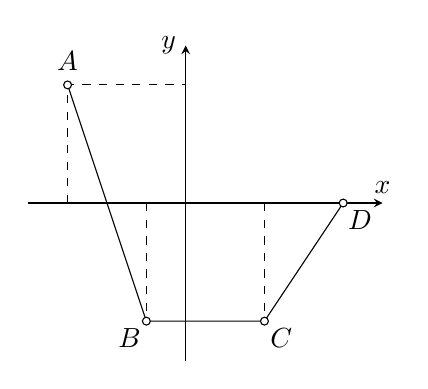
\begin{tikzpicture}[>=stealth]
			\draw[->](-2,0)--(5/2,0) node[above]{$x$};
			\draw[->](0,-2)--(0,2) node[left]{$y$};
			\draw[dashed](-3/2,0)--(-3/2,3/2)--(0,3/2) (-1/2,0)--(-1/2,-3/2) (1,0)--(1,-3/2);
			\path
			(0,0) coordinate (O)
			(-3/2,3/2) coordinate (A)
			(-1/2,-3/2) coordinate (B)
			(1,-3/2) coordinate (C)
			(2,0) coordinate (D);
			\draw (A)--(B)--(C)--(D);
			\foreach \x/\g in {A/90,B/-135,C/-45,D/-45} \draw[fill=white] (\x) circle (.05) + (\g:.3) node{$\x$};
		\end{tikzpicture}
	\end{center}
	\noindent(a) Tìm {\rm TXĐ} của hàm số $y$. (b) Tính $f(-3),f(-1),f(1),f(2),f(3),f(4)$. (c) Hàm số $y = f(x)$ đồng biến \& nghịch biến trong khoảng nào? (d) {\rm Đ{\tt/}S?} Khi xét $x_1 = 2$, $f(x_1) = f(2) = -3$, $x_2 = -3$, $f(x_2) = f(-3) = 3$, ta thấy $x_2 < x_1$, $f(x_2) > f(x_1)$ nên hàm số nghịch biến trong khoảng $[-3,2]$.
\end{baitoan}

\begin{baitoan}[\cite{Binh_boi_duong_Toan_9_tap_1}, 6.1., p. 53]
	Bảng sau ghi các giá trị tương ứng của 2 đại lượng $x,y$ phụ thuộc nhau.
	\begin{table}[H]
		\centering
		\begin{tabular}{|c|c|c|c|c|c|c|c|c|c|}
			\hline
			$x$ & 1 & 2 & 3 & 4 & 5 & 1 & 6 & 7 & 8 \\
			\hline
			$y$ & 0 & 2 & -1 & 5 & 4 & -4 & 3 & -2 & -6 \\
			\hline
		\end{tabular}
	\end{table}
	\noindent(a) $y$ có là hàm số của $x$ không? (b) $x$ có là hàm số của $y$ không? (c) Trường hợp là hàm số, nêu {\rm TXĐ}.
\end{baitoan}

\begin{baitoan}[\cite{Binh_boi_duong_Toan_9_tap_1}, 6.2., p. 53]
	Cho hàm số $y = f(x) = 3x^2 + 1$. (a) Tính $f(-1),f(0),f(1)$. (b) Tìm $x$ để $f(x) = 4$. (c) Trong 3 điểm $A(0,1),B(2,3),C(3,4)$, điểm nào không thuộc đồ thị hàm số đã cho?
\end{baitoan}

\begin{baitoan}[\cite{Binh_boi_duong_Toan_9_tap_1}, 6.3., p. 53]
	Bảng giá bán lẻ điện cho các hộ gia đình (chưa tính {\rm VAT}) (theo QĐ số 2256{\tt/}QĐ-BCT 12.3.2015 của Bộ Công thương):
	\begin{table}[H]
		\centering
		\begin{tabular}{|l|c|}
			\hline
			Mức độ sử dụng của mỗi hộ trong tháng & Giá bán điện (đồng{\tt/}kwh) \\
			\hline
			Bậc 1: cho kwh từ 0--50 & 1484 \\
			\hline
			Bậc 2: cho kwh từ 51--100 & 1533 \\
			\hline
			Bậc 3: cho kwh từ 101--200 & 1786 \\
			\hline
			Bậc 4: cho kwh từ 201--300 & 2242 \\
			\hline
			Bậc 5: cho kwh từ 301--400 & 2503 \\
			\hline
			Bậc 6: cho kwh từ 401 trở lên & 2587 \\
			\hline
		\end{tabular}
	\end{table}
	\noindent Gọi số điện sử dụng của hộ gia đình là $x$ {\rm kwh}, số tiền phải trả là $y$ đồng. (a) $y$ có phải là hàm số của $x$ không? (b) Nếu dùng hết $310$ {\rm kwh} điện thì phải trả bao nhiêu tiền?
\end{baitoan}

\begin{baitoan}[\cite{Binh_boi_duong_Toan_9_tap_1}, 6.4., p. 53]
	Chứng minh: (a) Hàm số $y = 2x + 3$ đồng biến trên $\mathbb{R}$. (b) Hàm số $y = -2x + 7$ nghịch biến trên $\mathbb{R}$.
\end{baitoan}

\begin{baitoan}[\cite{Binh_boi_duong_Toan_9_tap_1}, 6.5., p. 53]
	Cho $\Delta ABC$ đều có độ dài cạnh bằng $a$. Lấy $M\in AB$ sao cho $AM = x$ với $0 < x < a$. Vẽ hình chữ nhật MNPQ với $N\in AC$, $P,Q\in BC$. (a) Chứng minh diện tích hình chữ nhật MNPQ là hàm số của $x$. (b) Xác định $x$ để diện tích hình chữ nhật MNPQ lớn nhất.
\end{baitoan}

\begin{baitoan}[\cite{Binh_boi_duong_Toan_9_tap_1},  p. 53, Công thức Lorentz cho số cân nặng lý tưởng tương ứng với chiều cao]
	Cách đây hơn 1 thế kỷ, nhà khoa học người Hà Lan Hendrick Lorentz (1853--1928) đưa ra công thức tính số cân nặng lý tưởng của con người theo chiều cao:
	\begin{align*}
		\boxed{M = T - 100 - \dfrac{T - 150}{N}}
	\end{align*}
	trong đó $M$: số cân nặng {\rm kg}, $T$: chiều cao {\rm cm}, $N = 4$ với nam giới \& $N = 2$ với nữ giới. (a) Kiểm chứng công thức với cân nặng \& chiều cao của bản thân. (b) Viết công thức tính số cân nặng lý  tưởng của nam giới (ký hiệu là $P_1$) \& số cân nặng lý tưởng của nữ giới (ký hiệu là $P_2$) theo chiều cao. (c) Vẽ đồ thị hàm $M$ theo $T$. (d) $P_1,P_2$ có phải là hàm số của $T$ không? (c) Với $T$ bằng bao nhiêu thì $P_1 = P_2$?
\end{baitoan}

\begin{baitoan}[\cite{Tuyen_Toan_9_old}, VD16, p. 33]
	Cho hàm số $y = 2k(x - 1)^2 - kx(2x + 1) + 5x$ với tham số $k\ne1$. (a) Chứng minh $y$ là hàm số bậc nhất. (b) Với giá trị nào của $k$ thì hàm số đó là hàm số đồng biến? nghịch biến?
\end{baitoan}

\begin{baitoan}[\cite{Tuyen_Toan_9_old}, 98., p. 34]
	Cho hàm số $y = f(x) = 4x + 1 - \sqrt{3}(2x + 1)$. (a) Chứng minh $y$ là 1 hàm số bậc nhất đồng biến. (b) Tìm $x$ để $f(x) = 0$.
\end{baitoan}

\begin{baitoan}[\cite{Tuyen_Toan_9_old}, 99., p. 34]
	Xác định $k$ để hàm số $y = k(\sqrt{x} - 3)^2 + (k + 1)(\sqrt{x} + 2)^2$ là hàm số bậc nhất. Lúc đó $y$ là hàm số đồng biến hay nghịch biến?
\end{baitoan}

\begin{baitoan}[\cite{Tuyen_Toan_9_old}, 100., p. 34]
	Cho 2 hàm số $f(x) = mx - 2$, $g(x) = (m^2 + 1)x + 5$, trong đó $m\in\mathbb{R}^\star$. Chứng minh: (a) Hàm số $f(x) + g(x)$ là hàm số bậc nhất đồng biến. (b) Hàm số $f(x) - g(x)$ là hàm số bậc nhất nghịch biến. 
\end{baitoan}

\begin{baitoan}[\cite{Tuyen_Toan_9_old}, 101., p. 34]
	Cho hàm số $y = (m^2 - 4)x^2 - (2m + n)(5m - n)x - 3$. Với giá trị nào của $m,n$ thì $y$ là hàm số bậc nhất đồng biến? nghịch biến?
\end{baitoan}

\begin{baitoan}[\cite{Tuyen_Toan_9_old}, 102., p. 34]
	Cho hàm số $f(x) = 3x^2 + 1$. Chứng minh $f(x + 1) - f(x)$ là 1 hàm số bậc nhất.
\end{baitoan}

\begin{baitoan}[\cite{Tuyen_Toan_9_old}, 103., p. 34]
	Cho hàm số $y - f(x)$ . Biết $f(x - 1) = 3x - 5$. Chứng minh hàm số $y = f(x)$ là 1 hàm số bậc nhất.
\end{baitoan}

\begin{baitoan}[\cite{Tuyen_Toan_9_old}, 104., p. 34]
	Cho hàm số $y = ax + b$. Biết $f(1)\le f(2),f(5)\ge f(6),f(999) = 1000$. Tính $f(2010)$.
\end{baitoan}

%------------------------------------------------------------------------------%

\section{1st-Order Function \& Its Graph -- Hàm Số Bậc Nhất \& Đồ Thị Của Nó}

\begin{baitoan}[\cite{Tuyen_Toan_8}, VD36, p. 55]
	Cho hàm số $y = -\dfrac{1}{3}x$. (a) Vẽ đồ thị của hàm số đó. (b) Trong 3 điểm $A(-3,1),B(6,2),C(9,-3)$, điểm nào thuộc đồ thị (không vẽ 3 điểm đó)?
\end{baitoan}

\begin{baitoan}[\cite{Tuyen_Toan_8}, VD37, p. 55]
	Cho hàm số $y = 2k(x - 1)^2 - kx(2x + 1) + 5x$ với tham số $k\ne1$. (a) Chứng minh hàm số này là hàm số bậc nhất. (b) Với giá trị nào của $k\in\mathbb{R}$ thì hàm số đó là hàm số đồng biến? nghịch biến?
\end{baitoan}

\begin{baitoan}[\cite{Tuyen_Toan_8}, VD38, pp. 55--56]
	Cho hàm số $y = mx - 2m + 5$. (a) Vẽ đồ thị của hàm số khi $m = 3$. (b) Chứng minh với mọi giá trị của $m\in\mathbb{R}$, đồ thị của hàm số đã cho luôn đi qua 1 điểm cố định.
\end{baitoan}

\begin{baitoan}[\cite{Tuyen_Toan_8}, 219., p. 56]
	Vẽ đồ thị của hàm số $y = |x|$.
\end{baitoan}

\begin{baitoan}[\cite{Tuyen_Toan_8}, 220., p. 56]
	Vẽ đồ thị của hàm số $y = \dfrac{|x|}{x}$.
\end{baitoan}

\begin{baitoan}[\cite{Tuyen_Toan_8}, 221., p. 57]
	Cho 2 hàm số $y = f(x) = |2x|$ \& $y = g(x) = 3$. (a) Vẽ trên cùng 1 hệ trục tọa độ $Oxy$ đồ thị của 2 hàm số đã cho. (b) Dùng đồ thị tìm các giá trị của $x$ sao cho $|2x| < 3$.
\end{baitoan}

\begin{baitoan}[\cite{Tuyen_Toan_8}, 222., p. 57]
	Cho hàm số $y = f(x) = 4x + 1 - 3(x + 1)$. (a) Chứng minh $y$ là 1 hàm số bậc nhất đồng biến. (b) Tìm $x$ để $f(x) = 0$.
\end{baitoan}

\begin{baitoan}[\cite{Tuyen_Toan_8}, 223., p. 57]
	Xác định $k\in\mathbb{R}$ để hàm số $y = f(x) = (2k - 4)x^2 + (2k + 1)x + 13k + 4$ là hàm số bậc nhất. Khi đó, hàm số này là hàm số đồng biến hay nghịch biến?
\end{baitoan}

\begin{baitoan}[\cite{Tuyen_Toan_8}, 224., p. 57]
	Cho 2 hàm số $f(x) = mx - 2,g(x) = (m^2 + 1)x + 5$, trong đó $m\in\mathbb{R}^\star$. Chứng minh: (a) Hàm số $f(x) + g(x)$ là hàm số bậc nhất đồng biến. (b) Hàm số $f(x) - g(x)$ là hàm số bậc nhất nghịch biến.
\end{baitoan}

\begin{baitoan}[\cite{Tuyen_Toan_8}, 225., p. 57]
	Cho hàm số $f(x) = 3x^2 + 1$. Chứng minh $f(x + 1) - f(x)$ là 1 hàm số bậc nhất.
\end{baitoan}

\begin{baitoan}[\cite{Tuyen_Toan_8}, 226., p. 57]
	Cho hàm số $y = f(x)$. Biết $f(x - 1) = 3x - 5$, chứng minh hàm số $y = f(x)$ là 1 hàm số bậc nhất.
\end{baitoan}

\begin{baitoan}[\cite{Tuyen_Toan_8}, 227., p. 57]
	Xác định hàm số $y = ax + b$ biết đồ thị của nó cắt trục tung tại điểm A có tung độ bằng $-1$, cắt trục hoành tại điểm B có hoành độ bằng $3$.
\end{baitoan}

\begin{baitoan}[\cite{Tuyen_Toan_8}, 228., p. 57]
	Cho đường thẳng $(d):y = (m - 2)x - m + 4$. Chứng minh với mọi $m\in\mathbb{R}$ thì đường thẳng $(d)$ luôn đi qua 1 điểm cố định.
\end{baitoan}

\begin{baitoan}[\cite{Tuyen_Toan_8}, 229., p. 57]
	Cho 4 điểm $A(0,5),B(-3,0),C(1,1),M(-4.5,-2.5)$. (a) Chứng minh 3 điểm $A,B,M$ thẳng hàng, 3 điểm $A,B,C$ không thẳng hàng. (b) Tính diện tích của $\Delta ABC$.
\end{baitoan}

\begin{baitoan}[\cite{Tuyen_Toan_8}, 230., p. 57]
	Vẽ đồ thị của hàm số $y = |x - 1|$.
\end{baitoan}

\begin{baitoan}[\cite{Binh_boi_duong_Toan_9_tap_1}, H1, p. 55]
	$y$ là hàm số bậc nhất của $x\Leftrightarrow$: {\sf A.} $y = ax + b$, $a,b\in\mathbb{R}$. {\sf B.} $y = ax + b$, $a,b\in\mathbb{R}$, $ab\ne0$. {\sf C.} $y = ax + b$, $a,b\in\mathbb{R}$, $b\ne0$. {\sf D.} $y = ax + b$, $a,b\in\mathbb{R}$, $a\ne0$.
\end{baitoan}

\begin{baitoan}[\cite{Binh_boi_duong_Toan_9_tap_1}, H2, p. 55]
	Phân loại hàm số: (a) $y = \sqrt{2}(x - 1)$. (b) $y = \sqrt{2x} - 1$. (c) $y = \dfrac{x^2}{x} + 4$. (d) $y = \dfrac{2}{x} + 1$.
\end{baitoan}

\begin{baitoan}[\cite{Binh_boi_duong_Toan_9_tap_1}, H3, p. 56]
	Cho hàm số $y = (m + 1)x + 3m$. Khi đó: {\sf A.} $y$ là hàm số bậc nhất của biến $x$. {\sf B.} $y$ là hàm số bậc nhất của biến $m$. {\sf C.} $y$ là hàm số bậc nhất. {\sf D.} Với $m\ne-1$, $y$ là hàm số bậc nhất của biến $x$.
\end{baitoan}

\begin{baitoan}[\cite{Binh_boi_duong_Toan_9_tap_1}, H4, p. 56]
	Tìm điều kiện của $m$ để hàm số $y = (3m - 6)x + 8$ đồng biến trên $\mathbb{R}$.
\end{baitoan}

\begin{baitoan}[\cite{Binh_boi_duong_Toan_9_tap_1}, H5, p. 56]
	Vẽ đồ thị hàm số $y = -\dfrac{1}{2}x + 1$.
\end{baitoan}

\begin{baitoan}[\cite{Binh_boi_duong_Toan_9_tap_1}, VD1, p. 56]
	Với các giá trị nào của $m$ thì mỗi hàm số sau là hàm số bậc nhất? (a) $y = \sqrt{4 - m}(x - 1)$. (b) $y = \dfrac{m + 2}{m - 2}x + 3.5 + x$.
\end{baitoan}

\begin{baitoan}[\cite{Binh_boi_duong_Toan_9_tap_1}, VD2, p. 57]
	1 hình chữ nhật có 2 kích thước là {\rm10 cm, 15 cm}. Bớt mỗi kích thước của hình chữ nhật đi $x$ {\rm cm} với $0 < x < 10$. Gọi chu vi của hình chữ nhật mới là $y$ {\rm cm}. (a) Lập công thức tính chu vi $y$ của hình chữ nhật mới theo $x$. (b) Chứng minh $y$ là hàm số bậc nhất của $x$ \& vẽ đồ thị hàm số đó.
\end{baitoan}

\begin{baitoan}[\cite{Binh_boi_duong_Toan_9_tap_1}, VD3, p. 57]
	(a) Vẽ đồ thị 2 hàm số $y = x - 2$ \& $y = -x - 1$ trên cùng 1 mặt phẳng tọa độ. (a) 2 đường thẳng $y = -x - 1$ \& $y = x - 2$ cắt nhau tại C \& cắt trục $Ox$ theo thứ tự $A,B$. Tìm tọa độ của 3 điểm $A,B,C$. (c) Chứng minh $\Delta ABC$ vuông cân. (d) Tính chu vi \& diện tích $\Delta ABC$.
\end{baitoan}

\begin{baitoan}[\cite{Binh_boi_duong_Toan_9_tap_1}, VD4, p. 58]
	Cho hàm số $y = (2m + 1)x + m - 1$ với $m\ne-\dfrac{1}{2}$. (a) Xác định $m$ trong mỗi trường hợp: (i) Đồ thị hàm số đi qua $M(1,1)$. (ii) Đồ thị cắt trục tung, trục hoành lần lượt tại $A,B$ sao cho $\Delta OAB$ cân. (iii) Đồ thị cắt trục tung, trục hoành lần lượt tại $A,B$ sao cho $\Delta OAB$ có diện tích bằng $\dfrac{1}{2}$. (b) Tìm giá trị nguyên của $m$ để đồ thị cắt trục hoành tại điểm có hoành độ là số nguyên. (c) Tìm các điểm cố định mà đồ thị hàm số luôn đi qua với mọi giá trị của $m$.
\end{baitoan}

\begin{baitoan}[\cite{Binh_boi_duong_Toan_9_tap_1}, 7.1., p. 60]
	Cho 3 hàm số $y = 2x + 1$, $y = 4x$, $y = -2x + 5$ theo thứ tự có đồ thị là 3 đường thẳng $(d_1),(d_2),(d_3)$. (a) Trong 3 hàm số này, hàm số nào đồng biến, hàm số nào nghịch biến? (b) Vẽ $(d_1),(d_2),(d_3)$ trên cùng 1 mặt phẳng tọa độ. (c) Trong 4 điểm $A(1,3),B(0,4),C(-1,-4),D(-2,9)$ có điểm nào nằm trên $(d_1)$ hoặc $(d_2)$ hoặc $(d_3)$ không?
\end{baitoan}

\begin{baitoan}[\cite{Binh_boi_duong_Toan_9_tap_1}, 7.2., p. 61]
	Lập công thức biểu thị $y$ theo $x$. Cho biết công thức nào là hàm số bậc nhất (chỉ rõ $a,b$). (a) Diện tích tam giác $y$ $\rm cm^2$ có đáy là $x$ {\rm cm} \& chiều cao tương ứng là {\rm6 cm}. (b) Chu vi hình thoi $y$ {\rm cm} với cạnh là $x$ {\rm cm}. (c) Chu vi đường tròn $y$ {\rm cm} với bán kính là $x$ {\rm cm}. (d) Diện tích hình tròn $y$ $\rm cm^2$ với bán kính là $x$ {\rm cm}.
\end{baitoan}

\begin{baitoan}[\cite{Binh_boi_duong_Toan_9_tap_1}, 7.3., p. 61]
	Trong mặt phẳng tọa độ $Oxy$ cho 3 điểm $A(2,-1),B(-1,-7),C(3,1)$. (a) Viết phương trình đường thẳng BC. (b) Chứng minh 3 điểm $A,B,C$ thẳng hàng.
\end{baitoan}

\begin{baitoan}[\cite{Binh_boi_duong_Toan_9_tap_1}, 7.4., p. 61]
	Cho hàm số $y = (m - 2)x + 3$. (a) Với giá trị nào của $m$ thì hàm số đồng biến, nghịch biến, hàm hằng? (b) Xác định giá trị của $m$ để đồ thị hàm số đi qua điểm $A(1,4)$. (c) Vẽ đồ thị hàm số ứng với giá trị của $m$ tìm được ở (b).
\end{baitoan}

\begin{baitoan}[\cite{Binh_boi_duong_Toan_9_tap_1}, 7.5., p. 61]
	Cho 6 đường thẳng chứa 4 cạnh \& 2 đường chéo của 1 hình chữ nhật có tâm trùng với gốc tọa độ. Tìm số đường thẳng là đồ thị của 1 hàm số bậc nhất?
\end{baitoan}

\begin{baitoan}[\cite{Binh_boi_duong_Toan_9_tap_1}, 7.6., p. 61]
	Lập phương trình đường thẳng đi qua 2 điểm $A,B$ với: (a) $A(2,3),B(2,5)$. (b) $A(1,4),B(-5,4)$. (c) $A(2,2),B(-4,3)$. Từ đó đưa ra công thức tổng quát phương trình đường thẳng đi qua $A(x_1,y_1)$ \& $B(x_2,y_2)$.
\end{baitoan}

\begin{baitoan}[\cite{Binh_boi_duong_Toan_9_tap_1}, 7.7., p. 61]
	Cho 3 đường thẳng $(d_1):y = 1 - x$, $(d_2):x - y = 3$, $(d_3):(m + 1)x + (m - 1)y = 1 + 2m$. (a) Xác định $m$ để 3 đường thẳng cùng đi qua 1 điểm. (b) Chứng minh khi $m$ thay đổi, đường thẳng $(d_3)$ luông đi qua 1 điểm cố định.
\end{baitoan}

\begin{baitoan}[\cite{Binh_boi_duong_Toan_9_tap_1}, 7.8., p. 61]
	Cho hàm số $y = (m^2 + m + 1)x + 6$ có đồ thị $(d)$. (a) Chứng minh: $\forall m\in\mathbb{R}$, $y$ luôn là hàm số bậc nhất đồng biến. (b) Tìm $m$ để $(d)$ cắt $Ox$ tại A, cắt $Oy$ tại B sao cho: (i) Diện tích $\Delta AOB$ bằng $4$. (ii) Diện tích $\Delta AOB$ lớn nhất.
\end{baitoan}

\begin{baitoan}[\cite{Binh_boi_duong_Toan_9_tap_1}, p. 62, Mối quan hệ giữa độ F \& độ C]
	Độ Fahrenheit (độ {\rm F} hay ${}^\circ${\rm F}) là thang nhiệt được đặt theo tên nhà Vật lý người Đức Gabriel Fahrenheit (1686--1736) -- người đã đề xuất ra nó năm 1724. Theo đó, nước đóng bằng ở $32^\circ${\rm F} \& sôi ở $212^\circ${\rm F} (2 trạng thái này chênh lệch $180^\circ${\rm F}). Độ Celsius (độ {\rm C} hay ${}^\circ${\rm C}) là thang nhiệt được đặt theo tên nhà thiên văn học người Thụy Điển Anders Celsius (1701--1744) -- người đầu tiên đề nghị hệ thống đo nhiệt độ {\rm C} năm 1742 \& đến năm 1750, độ {\rm C} còn được gọi là độ bách phân. Theo đó, nước đóng băng ở $0^\circ${\rm C} \& sôi ở $100^\circ${\rm C}. Do đó, mỗi độ thuộc thang đo Celcius bằng $\dfrac{212 - 32}{100 - 0} = \dfrac{180}{100} = \dfrac{9}{5}$ độ thuộc thang đo Fahrenheit. Ngày nay, đa số các nước sử dụng thang nhiệt độ là độ {\rm C}, tuy nhiên 1 số nước, e.g., Mỹ, vẫn sử dụng nhiệt kế chia mức độ nhiệt độ theo độ {\rm F}. Mối quan hệ giữa số đo độ {\rm F}, ký hiệu là $T_{\rm F}$, \& số đo độ {\rm C}, ký hiệu là $T_{\rm C}$: $T_{\rm F} = 1.8TT_{\rm C} + 32$. (a) $T_{\rm F},T_{\rm C}$ có là hàm số bậc nhất có nhau không. (b) Xét tính đồng biến, nghịch biến của 2 hàm số này.
\end{baitoan}

\begin{baitoan}[\cite{Binh_boi_duong_Toan_9_tap_1}, VD1, p. 63]
	Xét sự biến thiên \& vẽ đồ thị hàm số $y = |2x + 3|$.
\end{baitoan}

\begin{baitoan}[\cite{Binh_boi_duong_Toan_9_tap_1}, VD2, p. 63]
	Cho hàm số $y = |x - 1| + |x - 5|$. (a) Vẽ đồ thị hàm số. (b) Xác định {\rm GTNN} của hàm số.
\end{baitoan}

\begin{baitoan}[\cite{Binh_boi_duong_Toan_9_tap_1}, p. 64]
	Xét sự biến thiên \& vẽ đồ thị hàm số: (a) $y = |-3x + 1|$. (b) $y = |x + 1| + |2x - 3|$.
\end{baitoan}

\begin{baitoan}[\cite{Tuyen_Toan_9_old}, VD17, p. 36]
	Cho hàm số $y = mx - 2m + 5$. (a) Vẽ đồ thị của hàm số với $m = 3$. (b) Chứng minh với mọi giá trị của $m$, đồ thị của hàm số đã cho luôn đi qua 1 điểm cố định.
\end{baitoan}

\begin{baitoan}[\cite{Tuyen_Toan_9_old}, 105., p. 37]
	Cho $A(x_1,y_1),B(x_2,y_2)$ là 2 điểm nằm trên đường thẳng $y = \sqrt{3}x + b$. Chứng minh $AB = 2|x_2 - x_1|$.
\end{baitoan}

\begin{baitoan}[\cite{Tuyen_Toan_9_old}, 106., p. 37]
	Xác định hàm số $y = ax + b$ biết đồ thị của nó cắt trục tung tại điểm A có tung độ bằng $-1$, cắt trục hoành tại điểm B có hoành độ bằng $3$.
\end{baitoan}

\begin{baitoan}[\cite{Tuyen_Toan_9_old}, 107., p. 37]
	Cho $A(0,5),B(-3,0),C(1,1),D(-4.5,-2.5)$. (a) Chứng minh 3 điểm $A,B,M$ thẳng hàng, \& 3 điểm $A,B,C$ không thẳng hàng. (b) Tính diện tích $\Delta ABC$.
\end{baitoan}

\begin{baitoan}[\cite{Tuyen_Toan_9_old}, 108., p. 37]
	Cho đường thẳng $(d):y = (m - 2)x - m + 4$. Chứng minh với mọi giá trị của $m$ thì đường thẳng $(d)$ luôn đi qua 1 điểm cố định.
\end{baitoan}

\begin{baitoan}[\cite{Tuyen_Toan_9_old}, 109., p. 37]
	Vẽ đồ thị của hàm số $y = \dfrac{1}{2}x + \dfrac{2\sqrt{x^2}}{x}$.
\end{baitoan}

\begin{baitoan}[\cite{Tuyen_Toan_9_old}, 110., p. 37]
	Vẽ đồ thị của hàm số: (a) $y = |x - 1|$. (b) $y = |x + 1| + \left|\dfrac{1}{2}x - 1\right|$.
\end{baitoan}

\begin{baitoan}[\cite{Tuyen_Toan_9_old}, 111., p. 37]
	Vẽ đồ thị của hàm số $y = \dfrac{x^3 + 2x^2 - x - 2}{x^2 + x - 2}$.
\end{baitoan}

\begin{baitoan}[\cite{Tuyen_Toan_9_old}, 112., p. 37]
	Cho điểm $A(-2,0)$ \& $(d)$ là đồ thị của hàm số $y = 2x - \dfrac{3x}{x}$. Qua điểm A có thể vẽ được bao nhiêu đường thẳng không cắt $(d)$?
\end{baitoan}

%------------------------------------------------------------------------------%

\section{Đường Thẳng Song Song \& Đường Thẳng Cắt Nhau. Hệ Số Góc Của Đường Thẳng $y = ax + b$, $a\ne0$}

\begin{baitoan}[\cite{Binh_boi_duong_Toan_9_tap_1}, H1, p. 66]
	Đồ thị hàm số $y = (\sqrt{5} - 2)x + 3$ cắt đồ thị hàm số: {\sf A.} $y =  \sqrt{5}x - 2x$. {\sf B.} $y = (\sqrt{5} - 1)x + 4 - x$. {\sf C.} $y = -2x + \sqrt{5}$. {\sf D.} $y = -2x + \sqrt{5}x + 2$.
\end{baitoan}

\begin{baitoan}[\cite{Binh_boi_duong_Toan_9_tap_1}, H2, p. 66]
	Cho 4 đường thẳng: $ (d_1):y = 1 - 5x$, $ (d_2):y = -5x + 2$, $(d_3): y = \dfrac{1}{5}x + \dfrac{1}{2}$, $(d_4):y = 3x + \dfrac{1}{3}$. {\rm Đ{\tt/}S?} (a) $(d_1)\bot(d_3)$. (b) $(d_1)\parallel(d_2)$. (c) $(d_1)\parallel(d_4)$. (d) $(d_2)$ cắt $(d_4)$.
\end{baitoan}

\begin{baitoan}[\cite{Binh_boi_duong_Toan_9_tap_1}, H3, p. 66]
	Tìm $m$ để 2 đường thẳng $(d_1):y = m^2x - 5$ \& $(d_2):y = 9x + 2m + 1$ song song với nhau.
\end{baitoan}

\begin{baitoan}[\cite{Binh_boi_duong_Toan_9_tap_1}, H4, p. 66]
	Tìm hệ số góc của đường thẳng $5x + 2y = 3$.
\end{baitoan}

\begin{baitoan}[\cite{Binh_boi_duong_Toan_9_tap_1}, VD1, p. 67]
	Cho 2 đường thẳng: $(d_1):y = (2m - 1)x + 2m - 3$, $(d_2):y = (m + 1)x + m$. Xác định $m$ để: (a) $(d_1)$ cắt $(d_2)$. (b) $(d_1)\parallel(d_2)$. (c) $(d_1)\bot(d_2)$.
\end{baitoan}

\begin{baitoan}[\cite{Binh_boi_duong_Toan_9_tap_1}, VD2, p. 67]
	Cho 2 đường thẳng $(d_1):y = x - 7$, $(d_2):y = -2x - 1$. Viết phương trình đường thẳng $(d)$ đi qua giao điểm của $(d_1)$ \& $(d_2)$ đồng thời song song với đường thẳng $(d_3):x - 2y + 1 = 0$.
\end{baitoan}

\begin{baitoan}[\cite{Binh_boi_duong_Toan_9_tap_1}, VD3, p. 68]
	Cho hàm số $y = (m - 1)x + m + 3$, $m$: tham số. Tìm giá trị của $m$ để đồ thị hàm số tạo với trục $Ox$ 1 góc bằng: (a) $60^\circ$. (b) $120^\circ$. (c) $\alpha^\circ$.
\end{baitoan}

\begin{baitoan}[\cite{Binh_boi_duong_Toan_9_tap_1}, VD4, p. 68]
	Cho 2 đường thẳng $(d_1):y = 3x + 2$, $(d_2):y = (2m^2 + 1)x + m + 1$. Xác định $m$ để $(d_1)$ song song với $(d_2)$. Khi đó xác định khoảng cách giữa chúng.
\end{baitoan}

\begin{baitoan}[\cite{Binh_boi_duong_Toan_9_tap_1}, VD5, p. 69]
	Cho $\Delta ABC$ vuông tại A, $AB = 3$ {\rm cm}, $AC = 4$ {\rm cm}. Trên cạnh BC lấy điểm M \& ký hiệu $BM = x$ {\rm cm}, $0 < x < 5$. Gọi $f(x)$ là diện tích của $\Delta ABM$, $g(x)$ là diện tích của $\Delta ACM$. (a) Chứng minh $f(x),g(x)$ là 2 hàm số bậc nhất của $x$. (b) Vẽ đồ thị 2 hàm số trên cùng 1 mặt phẳng tọa độ. (c) Gọi I là giao điểm của 2 đồ thị. Xác định tọa độ điểm I. Hoành độbiết \& tung độ của điểm I cho ta biết điều gì?
\end{baitoan}

\begin{baitoan}[\cite{Binh_boi_duong_Toan_9_tap_1}, VD6, p. 70]
	Trên mặt phẳng tọa độ $Oxy$ cho 3 điểm $A(-1,1),B(0,2),C(3,1)$. (a) Xác định tọa độ điểm D sao cho tứ giác ABCD là hình bình hành. (b) Chứng minh tứ giác ABCD là hình vuông.
\end{baitoan}

\begin{baitoan}[\cite{Binh_boi_duong_Toan_9_tap_1}, 8.1., p. 71]
	Nêu điều kiện để 3 đường thẳng $(d_1):y = a_1x + b_1$, $(d_2):y = a_2x + b_2$, $(d_3):y = a_3x + b_3$. (a) Song song với nhau. (b) Đôi một cắt nhau. (c) Đồng quy tại 1 điểm.
\end{baitoan}

\begin{baitoan}[\cite{Binh_boi_duong_Toan_9_tap_1}, 8.2., p. 71]
	Viết phương trình đường thẳng đi qua điểm $A(2,-3)$ \&: (a) Song song với đường thẳng $(d_1):y = 2x + 5$. (b) Vuông góc với đường thẳng $(d_2):y = -\dfrac{1}{3}x + 7$. (c) Đồng quy với 2 đường thẳng $(d_3):y = x - 1$ \& $(d_4):y = 3x + 5$.
\end{baitoan}

\begin{baitoan}[\cite{Binh_boi_duong_Toan_9_tap_1}, 8.3., p. 71]
	2 đường thẳng $(d):4mx + 3y = -2$ \& $(d'):2my = nx - 2$ cắt nhau tại điểm $M(1,-2)$. Tìm hệ số góc của mỗi đường thẳng $(d),(d')$.
\end{baitoan}

\begin{baitoan}[\cite{Binh_boi_duong_Toan_9_tap_1}, 8.4., p. 71]
	(a) Viết phương trình đường thẳng $(d)$ đi qua 2 điểm $A(2,-1),B\left(\dfrac{1}{2},2\right)$. (b) Chứng minh 3 điểm $A,B,C(5,-7)$ thẳng hàng. (c) Với giá trị nào của $m$ thì đồ thị của 2 hàm số $y = mx + 5$, $y = 3x - 7$, \& đường thẳng $(d)$ đồng quy?
\end{baitoan}

\begin{baitoan}[\cite{Binh_boi_duong_Toan_9_tap_1}, 8.5., p. 71]
	(a) Viết phương trình đường thẳng đi qua điểm $A(-3,2)$ \& song song với đường thẳng $y = 3x - 5$. (b) Tính khoảng cách giữa 2 đường thẳng song song đó.
\end{baitoan}

\begin{baitoan}[\cite{Binh_boi_duong_Toan_9_tap_1}, 8.6., p. 71]
	Trên mặt phẳng tọa độ $Oxy$ cho 3 điểm $A(-3,2),B(-1,-1),C(2,0)$. (a) Viết phương trình đường thẳng chứa 3 cạnh của $\Delta ABC$. (b) Viết phương trình đường cao $AD,BE,CF$ của $\Delta ABC$. (c) Tìm tọa độ trực tâm H của $\Delta ABC$.
\end{baitoan}

\begin{baitoan}[\cite{Binh_boi_duong_Toan_9_tap_1}, 8.7., p. 71]
	Cho 2 hàm số bậc nhất với $m$: tham số, $y = (m + 1)x + 2m - 1$, $y = (2m - 3)x + 3m - 6$. (a) Xác định giá trị của $m$ để đồ thị của chúng: (i) Song song với nhau. (ii) Cắt nhau tại 1 điểm trên trục tung. (iii) Cắt nhau tại 1 điểm nằm ở bên phải tung. (b) Chứng minh khi $m$ thay đổi thì đồ thị của mỗi hàm số trên đều đi qua 1 điểm cố định.
\end{baitoan}

\begin{baitoan}[\cite{Binh_boi_duong_Toan_9_tap_1}, 8.8., p. 71]
	Cho 3 đường thẳng $(d_1):y = 4x,(d_2):y = x + 3,(d_3):y = -x + 5$. (a) Chứngm inh $(d_1),(d_2),(d_3)$ cắt nhau tại 1 điểm A. Xác định tọa độ điểm A. (b) Gọi B là giao điểm của $(d_2)$ với trục hoành, C là giao điểm của $(d_3)$ với trục hoành. Chứng minh $\Delta ABC$ vuông cân.
\end{baitoan}

\begin{baitoan}[\cite{Binh_boi_duong_Toan_9_tap_1}, p. 72, Phương trình đường thẳng đi qua 2 điểm cho trước]
	Cho 2 điểm $A(x_1,y_1),B(x_2,y_2)$. Chứng minh: (a) Nếu $x_1\ne x_2,y_1\ne y_2$ thì đường thẳng AB cắt 2 trục tọa độ \& có phương trình $\dfrac{x - x_1}{x_2 - x_1} = \dfrac{y - y_1}{y_2 - y_1}$. (b) Nếu $x_1 = x_2,y_1\ne y_2$ thì đường thẳng $AB\bot Ox$, cắt trục $Ox$ tại điểm có hoành độ $x_1$ \& có phương trình $x = x_1$ ($= x_2$). (c) Nếu $x_1\ne x_2,y_1 = y_2$ thì đường thẳng $AB\bot Oy$, cắt trục $Ox$ tại điểm có tung độ $y_1$ \& có phương trình $y = y_1$ ($= y_2$).
\end{baitoan}

\begin{baitoan}[\cite{Tuyen_Toan_9_old}, VD18, p. 38]
	Cho 2 đường thẳng $(d_1):y = mx - 2(m + 2)$ với $m\ne0$, $(d_2):y = (2m - 3)x + m^2 - 1$ với $m\ne\dfrac{3}{2}$. (a) Chứng minh với mọi giá trị của $m$, 2 đường thẳng $(d_1),(d_2)$ không thể trùng nhau. (b) Tìm các giá trị của $m\in\mathbb{R}$ để: (i) $(d_1)\parallel(d_2)$. (ii) $(d_1)$ cắt $(d_2)$. (iii) $(d_1)\bot(d_2)$.
\end{baitoan}

\begin{baitoan}[\cite{Tuyen_Toan_9_old}, 113., pp. 39--40]
	Cho 3 đường thẳng: $(d_1):y = -2x + 3$, $(d_2):y = -2x + m$, $(d_3):y = \dfrac{1}{2}x + 1$. Không vẽ 3 đường thẳng này, cho biết vị trí tương đối của chúng đối với nhau.
\end{baitoan}

\begin{baitoan}[\cite{Tuyen_Toan_9_old}, 114., p. 40]
	Cho 3 đường thẳng: $(d_1):y = (2m + 1)x - (2m + 3)$ với $m\ne-\dfrac{1}{2}$, $(d_2):y = (m - 1)x + m$ với $m\ne1$. Tìm giá trị của $m$ để: (a) $(d_1)$ cắt $(d_2)$. (b) $(d_1)\parallel(d_2)$. (c) $(d_1)\bot(d_2)$.
\end{baitoan}

\begin{baitoan}[\cite{Tuyen_Toan_9_old}, 115., p. 40]
	Cho điểm $A(3,2)$. Viết phương trình đường thẳng $(d)$ đi qua A \& vuông góc với OA. Tính góc tạo thành bởi đường thẳng $(d)$ \& trục $Ox$.
\end{baitoan}

\begin{baitoan}[\cite{Tuyen_Toan_9_old}, 116., p. 40]
	Cho 3 đường thẳng: $(d_1):y = -3x$, $(d_2):y = 2x + 5$, $(d_3):y = x + 4$. Chứng minh 3 đường thẳng này đồng quy.
\end{baitoan}

\begin{baitoan}[\cite{Tuyen_Toan_9_old}, 117., p. 40]
	Tìm giá trị của $m$ để 3 đường thẳng sau đồng quy: $(d_1):y = x - 4$, $(d_2):y = -2x - 1$, $(d_3):y = mx + 2$.
\end{baitoan}

\begin{baitoan}[\cite{Tuyen_Toan_9_old}, 118., p. 40]
	Tìm diện tích hình giới hạn bởi 3 đường thẳng: $(d_1):y = \dfrac{1}{3}x$, $(d_2):y = -3x$, $(d_3):y = -x + 4$.
\end{baitoan}

%------------------------------------------------------------------------------%

\section{Miscellaneous}

\begin{baitoan}[\cite{Tuyen_Toan_9_old}, VD19, p. 41]
	Cho 3 đường thẳng: $(d_1):y = (m^2 - 1)x + (m^2 - 5)$ với $m\ne\pm1$, $(d_2):y = x + 1$, $(d_3):y = -x + 3$. (a) Chứng minh khi $m$ thay đổi thì $(d_1)$ luôn đi qua 1 điểm cố định. (b) Chứng minh nếu $(d_1)\parallel(d_3)$ thì $(d_1)\bot(d_3)$. (c) Xác định $m$ để 3 đường thẳng $(d_1),(d_2),(d_3)$ đồng quy.
\end{baitoan}

\begin{baitoan}[\cite{Tuyen_Toan_9_old}, 119., p. 42]
	Cho hàm số $y = f(x)$ nghịch biến trong khoảng $(0,1)$. Biết $f\left(\dfrac{\sqrt{2}}{2}\right) = 0$. Chứng minh: (a) $f(\sqrt{3} - \sqrt{2}) > 0$. (b) $f\left(\sqrt{2} - \dfrac{\sqrt{2}}{3}\right) < 0$. (c) Xét dấu của $y$.
\end{baitoan}

\begin{baitoan}[\cite{Tuyen_Toan_9_old}, 120., p. 42]
	Trong mặt phẳng tọa độ, cho điểm $A(x,y)$ trong đó $x = m + 2$, $y = 3m - 1$ với $m\in\mathbb{R}$. Tìm tập hợp các điểm A.
\end{baitoan}

\begin{baitoan}[\cite{Tuyen_Toan_9_old}, 121., p. 42]
	Xác định hàm số $y = ax + b$ biết đồ thị của nó đi qua điểm $A(1,2)$ \& vuông góc với đồ thị của hàm số $y = \dfrac{1}{3}x - 1$.
\end{baitoan}

\begin{baitoan}[\cite{Tuyen_Toan_9_old}, 122., p. 42]
	Dùng đồ thị để: (a) Giải phương trình $|x| = -\dfrac{1}{2}x + \dfrac{3}{2}$. (b) Chứng minh phương trình $|x| = x - 2$ vô nghiệm.
\end{baitoan}

\begin{baitoan}[\cite{Tuyen_Toan_9_old}, 123., p. 42]
	Cho 2 đường thẳng: $(d_1): y = mx - 5$, $(d_2):y = -3x + 1$. (a) Xác định tọa độ giao điểm A của $(d_1)$ \& $(d_2)$ khi $m = 3$. (b) Xác định giá trị của $m$ để $M(3,-8)$ là giao điểm của $(d_1),(d_2)$.
\end{baitoan}

\begin{baitoan}[\cite{Tuyen_Toan_9_old}, 124., p. 42]
	Cho 2 đường thẳng: $(d_1):y = 4mx - (m + 5)$ với $m\ne0$, $(d_2):y = (3m^2 + 1)x + (m^2 - 4)$. (a) Chứng minh khi $m$ thay đổi thì đường thẳng $(d_1)$ luôn đi qua 1 điểm A cố định, đường thẳng $(d_2)$ luôn đi qua 1 điểm B cố định. (b) Tính khoảng cách AB. (c) Với giá trị nào của $m$ thì $(d_1)\parallel(d_2)$? (d) Với giá trị nào của $m$ thì $(d_1)$ cắt $(d_2)$? Tìm tọa độ giao điểm khi $m = 2$ \& cho $m$ tổng quát.
\end{baitoan}

\begin{baitoan}[\cite{Tuyen_Toan_9_old}, 125., p. 42]
	Cho điểm $A(0,-1),B(-4,3)$. Viết phương trình đường thẳng $(d)$ là đường trung trực của AB. Tính góc $\alpha$ tạo bởi đường thẳng $d$ với tia $Ox$.
\end{baitoan}

%------------------------------------------------------------------------------%

\printbibliography[heading=bibintoc]
	
\end{document}